\documentclass[11pt,twoside]{scrartcl}
%\documentclass[11pt,twoside]{article}

%opening
\newcommand{\lecid}{15-316}
\newcommand{\leccourse}{Software Foundations of Security and Privacy}
\newcommand{\lecdate}{} %e.g. {October 21, 2013}
\newcommand{\lecnum}{5}
\newcommand{\lectitle}{Memory Safety \& Sandboxing}
\newcommand{\lecturer}{Matt Fredrikson}
\newcommand{\lecurl}{https://15316-cmu.github.io/index}

\usepackage{varwidth}
\usepackage{lecnotes}
\usepackage[irlabel]{bugcatch}

\usepackage{tikz}
\usetikzlibrary{automata,shapes,positioning,matrix,shapes.callouts,decorations.text,patterns,trees,backgrounds}

% \usepackage[bracketinterpret,seqinfers,sidenotecalculus]{logic}
% \newcommand{\I}{\interpretation[const=I]}

% \newcommand{\bebecomes}{\mathrel{::=}}
% \newcommand{\alternative}{~|~}
% \newcommand{\asfml}{F}
% \newcommand{\bsfml}{G}
% \newcommand{\cusfml}{C}
% \def\leftrule{L}%
% \def\rightrule{R}%

\begin{document}

\newcommand{\atrace}{\sigma}%
%% the standard interpretation naming conventions
\newcommand{\stdI}{\dTLint[state=\omega]}%
\newcommand{\Ip}{\dTLint[trace=\atrace]}%
\newcommand{\ws}{\omega}\newcommand{\wt}{\nu}% 

\maketitle
\thispagestyle{empty}

%%%%%%%%%%%%%%%%%%%%%%%%%%%%%%%%%%%%%%%%%%%%%%

\section{Introduction \& Recap}

In the previous lecture we looked into proving that programs satisfy safety properties given as formulas in the first-order dynamic logic. In particular, we can write contract properties with precondition $\ausfml$ and postconditions $\busfml$ for a program $\asprg$ as:
\begin{equation}
\ausfml \limply \dbox{\asprg}{\busfml}
\end{equation}
If this formula is valid, then it means that in every state $\omega$, if $\omega\models\ausfml$ then after all terminating runs of $\asprg$ starting in $\omega$ the final state $\nu\models\busfml$. 

So far the programs that we have studied are not too interesting when it comes to concerns about security---they can perform operations over integers, but they can't interact with memory or arrays. 
Today we will start by extending our language to support pointer operations over memory, and then discuss \emph{memory safety} as well as a more flexible mechanism for policy enforcement called \emph{software fault isolation}. Importantly, we will build on our understanding of sound axioms and proof rules to justify the correctness of this mechanism.

\section{Memory Safety}

While most imperative programming languages support convenient dynamic memory allocation and access with syntax like \verb'malloc' and \verb'a[i]', at the end of the day this is nothing more than syntactic sugar for managing a large integer-indexed array of values. We can add basic support for this to our language by introducing pointers, and adding an integer-indexed memory to our program state. Now terms in our language will have the following syntax.
\begin{equation}
\label{def:term-syntax}
  \astrm,\bstrm ~\bebecomes~
  x
  \alternative
  c
  \alternative
  \astrm+\bstrm
  \alternative
  \astrm\cdot\bstrm
  \alternative
  \pderef{\astrm}
\end{equation}
The term $\pderef{\astrm}$ denotes the value obtained by evaluating $\astrm$ in the current state, and accessing the memory at the corresponding index. This takes care of reading from the memory array, now we add support for updating memory by introducing a new type of program command.
\begin{equation}
\label{def:program-syntax}
  \asprg,\bsprg ~\bebecomes~
  \pupdate{\pumod{x}{\astrm}}
  \alternative
  \pupdate{\pumod{\pderef{\astrm}}{\bstrm}}
  \alternative
  \passert{\ivr}
  \alternative
  \pif{\ivr}{\asprg}{\bsprg}
  \alternative
  \asprg;\bsprg
  \alternative
  \pwhile{\ivr}{\asprg}
\end{equation}
The command $\pupdate{\pumod{\pderef{\astrm}}{\bstrm}}$ evaluates $\astrm$ and $\bstrm$ in the current state, and sets the value of memory indexed at the value of $\astrm$ to the value of $\bstrm$.

Now for the semantics. We will need to track the value of variables as we did before with a mapping from variables to values. But we will also need to track the state of the memory, which we will formalize as a partial mapping from non-negative integers to values. Real machines don't have unlimited memory, which is why the mapping is partial: we assume that the memory can hold at most \maxmem values, so the mapping is only defined on $0 \le i \le \maxmem$. 

We will continue to denote states by $\omega$, and write $\omega_V(x)$ to refer to the value of the variable mapping, and $\omega_M(x)$ to refer to the memory array. The semantics of terms can now be defined as follows.
\begin{definition}[Semantics of terms]
\label{def:term-semantics}
The \emph{semantics of a term} $\astrm$ in a state $\omega$ is its value $\omega\llbracket\astrm\rrbracket$.
It is defined inductively by distinguishing the shape of term $\astrm$ as follows:
\begin{itemize}
  \item \m{\omega\llbracket x\rrbracket = \omega_V(x)} for variable $x$
  \item \m{\omega\llbracket c\rrbracket = c} for number literals $c$
  \item \m{\omega\llbracket\astrm\odot\bstrm\rrbracket = \omega\llbracket\astrm\rrbracket \odot \omega\llbracket\bstrm\rrbracket}, where $\odot \in \{+,\times\}$
  \item \m{\omega\llbracket\pderef{\astrm}\rrbracket = \omega_M(\omega\llbracket\astrm\rrbracket)} if $0 \le \omega\llbracket\astrm\rrbracket < \maxmem$, else undefined
\end{itemize}
\end{definition}
Adding pointers to our language has led to a complication: now terms can be undefined. Specifically, if $\astrm$ evaluates to a negative number, or a number larger than the maximum memory size \maxmem, then the term $\pderef{\astrm}$ is not defined.

This complication manifests in how we define the semantics of formulas. Because terms can now be undefined in certain states, we need to account for this in the semantics of formulas that might include terms. Whenever a term in a formula is undefined in a particular state, then the value of the formula is as well.

\begin{definition}[Semantics of arithmetic formulas] \label{def:arithmetic-semantics}
The DL formula $\asfml$ is true in state $\iportray{\I}$, written \(\imodels{\I}{\asfml}\), as inductively defined by distinguishing the shape of formula $\asfml$:
\begin{enumerate}
\item \(\inonmodels{\I}{\mfalse}\), i.e., \mfalse is true in no states
\item \(\imodels{\I}{\mtrue}\), i.e., \mtrue is true in all states
\item \(\imodels{\I}{\astrm=\bstrm}\) iff \(\ivaluation{\I}{\astrm}=\ivaluation{\I}{\bstrm}\) and both terms are defined in $\omega$.
\item \(\imodels{\I}{\astrm\leq\bstrm}\) iff \(\ivaluation{\I}{\astrm}\leq\ivaluation{\I}{\bstrm}\) and both terms are defined in $\omega$.
\item \(\imodels{\I}{\asfml\land\bsfml}\) iff \(\imodels{\I}{\asfml}\) and \(\imodels{\I}{\bsfml}\) if $P$ and $Q$ are defined in $\omega$.
\item \(\imodels{\I}{\asfml\lor\bsfml}\) iff \(\imodels{\I}{\asfml}\) or \(\imodels{\I}{\bsfml}\)  if $P$ and $Q$ are defined in $\omega$.
\item \(\imodels{\I}{\lnot\asfml}\) iff \(\inonmodels{\I}{\asfml}\) if $P$ is defined in $\omega$.
\item \(\imodels{\I}{\asfml\limply\bsfml}\) iff \(\inonmodels{\I}{\asfml}\) or \(\imodels{\I}{\bsfml}\) and $P$ and $Q$ are defined in $\omega$.
\item \(\imodels{\I}{\asfml\lbisubjunct\bsfml}\) iff both are true or both false and $P$ and $Q$ are defined in $\omega$.
\end{enumerate}
\end{definition}

Finally, we get to the semantics of programs. Obviously we need to add a new definition for the memory update command $\pupdate{\umod{\pderef{\astrm}}{\bstrm}}$. But programs may contain terms and formulas, which we now know can be undefined in some states. We define the semantics of a program with a term or formula that is undefined in a state as aborting in the next subsequent state.

First some notation.
If $\omega_M$ is a memory in state $\omega$, then we write $\memupd{\omega_M}{\astrm}{\bstrm}$ to denote the new memory obtained by copying $\omega_M$, and changing its mapping at $\omega\llbracket\astrm\rrbracket$ to map to $\omega\llbracket\bstrm\rrbracket$. So suppose that $\omega_M(0) = 1, \omega_M(1) = 2$. Then $\memupd{\omega_M}{1}{3}(0) = 1$ and  $(\memupd{\omega_M}{1}{3})(1) = 3$. We can apply this update notation multiple times, so that:
\[
\memupd{\memupd{\omega_M}{1}{3}}{0}{4}(0) = 4, \memupd{\memupd{\omega_M}{1}{3}}{0}{4}(1) = 3
\]
We'll adopt the convention that the rightmost update to a particular index is the one that we use when looking up values. So for example,
\[
\memupd{\memupd{\omega_M}{1}{3}}{1}{4}(1) = 4
\]

\begin{definition}[Trace semantics of programs] \label{def:program-trace}
  % \newcommand{\ws}{\omega}\newcommand{\wt}{\nu}% 
  % \renewcommand{\I}{\iconcat[state=\ws]{\stdI}}%
  % \renewcommand{\It}{\iconcat[state=\wt]{\stdI}}%
  
The \dfn[valuation!of~programs]{trace semantics $\iaccess[\alpha]{\I}$ of a program}~$\alpha$ is the set of all its possible traces and is defined inductively as follows:
    % \index{_\tau(\alpha)_@$\tau(\alpha)$}%
    \begin{enumerate}
    \item
      \m{\iaccess[\pupdate{\umod{x}{\astrm}}]{\I}}
      =
      \begin{tabular}{l}
      \(\{(\iget[state]{\I},\iget[state]{\It}) \with \omega\llbracket\astrm\rrbracket~\text{is defined and}~
      \iget[state]{\It}=\iget[state]{\I}~\text{except that}~ \nu_V(x)=\ivaluation{\I}{\astrm}\}\ \cup\) 
      \\
      \(\{(\iget[state]{\I},\errstate) \with \omega\llbracket\astrm\rrbracket~\text{is not defined}\}\)
      \end{tabular}

  \item \m{\iaccess[\pupdate{\umod{\pderef{\astrm}}{\bstrm}}]{\I}}
          =
          \begin{tabular}{l}
          \(\{(\omega,\nu) \with 0 \le \omega\llbracket\astrm\rrbracket \le \maxmem, \omega\llbracket\bstrm\rrbracket~\text{defined}, \nu_M = \memupd{\omega_M}{\omega\llbracket\astrm\rrbracket}{\omega\llbracket\bstrm\rrbracket}\}\ \cup\) \\
          \(\{(\iget[state]{\I},\errstate) \with \lnot(0 \le \omega\llbracket\astrm\rrbracket \le \maxmem)~\text{or}~\omega\llbracket\bstrm\rrbracket~\text{not defined}\}\)
          \end{tabular}
   
   \item \(\iaccess[\passert{\ivr}]{\I}\)
      =
      \begin{tabular}{l}
      \(\{(\ws,\ws) \with \omega\llbracket\astrm\rrbracket~\text{is defined and}~
      \imodels{\I}{\ivr}\} \cup\) \\
      \(\{(\ws,\errstate) \with \omega\models\ivr~\text{is not defined or}~
      \inonmodels{\I}{\ivr}\}\)
      \index{$\ptest{}$}
      \end{tabular}
    
    \item \(\iaccess[\pif{\ivr}{\alpha}{\beta}]{\I}\) =
      \begin{tabular}{l}
      \(\{\atrace \in \iaccess[\alpha]{\I} \with \atrace_0\llbracket\astrm\rrbracket~\text{is defined and}~\atrace_0 \models \ivr\}\ \cup\) \\
      \(\{\atrace \in \iaccess[\beta]{\I} \with \atrace_0\llbracket\astrm\rrbracket~\text{is defined and}~\atrace_0 \nonmodels \ivr\}\ \cup\) \\
      \(\{(\omega,\errstate) \with \omega\models\ivr~\text{is not defined}\}\)
      \end{tabular}
    
    \item \(\iaccess[{\alpha};{\beta}]{\I} =
      \{\atrace \compose \varsigma \with \atrace\in\iaccess[\alpha]{\I} \mand \varsigma\in\iaccess[\beta]{\I}\}\);\\
      the composition of~\m{\atrace=(\atrace_0,\atrace_1,\atrace_2,\dots)} and~\m{\varsigma=(\varsigma_0,\varsigma_1,\varsigma_2,\dots)} is
      \[
      \atrace \compose \varsigma \eqdef
      \begin{cases}
        (\atrace_0,\dots,\atrace_n,\varsigma_1,\varsigma_2,\dots) &\mylpmi[\text{if}~] \text{$\atrace$ terminates in $\atrace_n$}~\text{and}~\atrace_n=\varsigma_0\\
        \atrace &\mylpmi[\text{if}~] \atrace~\text{does not terminate}
      \end{cases}
      \]
    
    \item \(\iaccess[\pwhile{\ivr}{\alpha}]{\I}\)
      =
      \begin{tabular}{l}
        \(\{\atrace^{(0)} \compose \dots \compose \atrace^{(n)} \with\)
          for all $0\leq i\leq n$:
          $\atrace^{(i)}_0 \models \ivr$,
          $\atrace^{(i)} \in \iaccess[\asprg]{\Iz[i]}$, and \\
          \ \ $\atrace^{(n)}$ either doesn't terminate, or terminates with $\atrace^{(n)}_m \nonmodels \ivr\}~\cup$
        \\
        \(\{\atrace^{(0)} \compose \atrace^{(1)} \compose \atrace^{(2)} \compose \dots \with\)
          for all $i\in\naturals$:
          \m{\atrace^{(i)}_0 \models \ivr},
          \m{\atrace^{(i)} \in \iaccess[\asprg]{\Iz[i]}}$\}~\cup$
        \\
        \(\{(\iget[state]{\I}) \with \inonmodels{\I}{\ivr}\}~\cup\)
        \\
        \(\{\atrace^{(0)} \compose \dots \compose \atrace^{(n)} \compose (\Lambda) \with\)
          for all $0\leq i \leq n$:
          $\atrace^{(i)}_0 \models \ivr$,
          $\atrace^{(i)} \in \iaccess[\asprg]{\Iz[i]}$, and \\
          \ \ $\atrace^{(n)}$ terminates with $\atrace^{(n)}_m \models \ivr$ not defined$\}~\cup$
        \\
        \(\{(\omega,\Lambda) \with \omega \models \ivr~\text{not defined}\}\)
      \end{tabular}
    \end{enumerate}
\end{definition}
While it may be tedious to track the presence of undefined terms and formulas through the evaluation of a program, we will see that this is central to the very definition of what memory safety means for a particular programming language.

\paragraph{Axioms and Proof Rules.}
Now we have semantics for programs with pointers and indexed memory, the next logical thing to do is find some useful axioms to help us reason about them. 

Just as we had an axiom for assignment to variables, we have a similar axiom for updates to a pointer. But in the assignment axiom, we performed a syntactic substitution of the target variable in the postcondition. In this case we can readily see that looking for mere occurrences of a pointer expression will not suffice. Consider the following:
\begin{equation}
\dbox{x:=1;y:=1;\pderef{x}:=0}{\pderef{y}\ne0}
\end{equation}
After executing the first two assignments, $\pderef{x}$ and $\pderef{y}$ point to the same memory location. So if we tried to close out a proof like the following:
\begin{sequentdeduction}
\linfer[assignb] {
  \lsequent{\pderef{y}\ne0,x=1,y=1}{\pderef{y}\ne0}
} {
  \lsequent{\pderef{y}\ne0,x=1,y=1}{\dbox{\pderef{x}:=0}{\pderef{y}\ne0}}
}
\end{sequentdeduction}
then we would be misled to say the least. Rather, we need to make sure that the update is reflected in any subsequent memory read to the same address, regardless of the syntactic form of the index term. Perhaps something like the following:
\begin{equation}
\label{eq:halfaxiom}
\dbox{\pderef{\astrm}:=\bstrm}{p(\pderefop)}
\lbisubjunct
p(\memupd{\pderefop}{\astrm}{\bstrm})
\end{equation}
Now when we repeat the derivation from before,
\begin{sequentdeduction}
\linfer {
  \lsequent{\pderef{y}\ne0,x=1,y=1}{\memupd{\pderefop}{x}{0}(y)\ne0}
} {
  \lsequent{\pderef{y}\ne0,x=1,y=1}{\dbox{\pderef{x}:=0}{\pderef{y}\ne0}}
}
\end{sequentdeduction}
there is no way to close out the proof because $x=y$ and $\memupd{\pderefop}{x}{0}(y) = 0$. But this proof rule isn't sound, because what if $\astrm$ evaluates to an out-of-bounds value? 
We need to add an assertion that the value of $\astrm$ is within the correct range. This leads to the \irref{mwrite} axiom, which combines Equation~\ref{eq:halfaxiom} with the in-bounds check.
\[
\cinferenceRule[mwrite|$\dibox{*}_{=}$]{mwrite}
{\linferenceRule[equiv]
  {p(\memupd{\pderefop}{\astrm}{\bstrm}) \land 0 \le \astrm < \maxmem}
  {\axkey{\dbox{\pderef{\astrm}:=\bstrm}{p(\pderefop)}}}
}{}%
\]
Axiom \irref{mwrite} takes care of what to do when we update memory, but we also need a way to reason about reads from memory. If we only ever reason about programs that never update memory, then this is easy because anything we need to know about its value at particular indices is already in our assumptions. We can then work with the index like we would any other value mentioned in a program.

But what about programs that update memory and then read from it afterwards? There are two cases to cover: reading from an index that was previously written to, and reading from one that was not. In the first case, we have some memory $\memupd{\pderefop}{\astrm}{\bstrm}$ and we perform an access $\memupd{\pderefop}{\astrm}{\bstrm}(\astrm')$ where $\astrm = \astrm'$ in the current state. Then the value that is read from memory will be $\bstrm$. But of course we also need to make sure that we are reading from an index in the appropriate range. This is captured in the \irref{mreadeq} rule.
\[
\cinferenceRule[mreadeq|$\dibox{*}_{1}$]{mreadeq}
{\linferenceRule[sequent]
  {
    \lsequent{\Gamma}{\astrm=\astrm'}
    &\lsequent{\Gamma}{0 \le \astrm' < \maxmem}
  }
  {\lsequent{\Gamma}{\memupd{\pderefop}{\astrm}{\bstrm}(\astrm')=\bstrm}}
}{}%
\]
Note that because we must prove that $\astrm = \astrm'$ in this case, for the right premise it is fine to alternatively prove that $\lsequent{\Gamma}{0 \le \astrm U}$ for the right premise, as this will not affect soundness.
In the case where $\astrm\ne\astrm'$, we use similar reasoning to conclude that $\memupd{\pderefop}{\astrm}{\bstrm}(\astrm')$ takes whatever the value at index $\astrm'$ in $\pderefop$ was \emph{before} the update, i.e. $\pderef{\astrm'}$. This gives us the \irref{mreadneq} rules.
\[
\cinferenceRule[mreadneq|$\dibox{*}_{2}$]{mreadneq}
{\linferenceRule[sequent]
  {
    \lsequent{\Gamma}{\astrm\ne\astrm'}
    &\lsequent{\Gamma}{0 \le \astrm' < \maxmem}
  }
  {\lsequent{\Gamma}{\memupd{\pderefop}{\astrm}{\bstrm}(\astrm')=\pderef{\astrm'}}}
}{}%
\]
The axiom \irref{mwrite} and rules \irref{mreadeq}, \irref{mreadneq} are sufficient to prove safety properties about programs with pointer operations. 

\paragraph{A syntactical sidenote.}
The axiom and rules that we introduced ask us to explicitly keep track of the updates that occur as we work through a dynamic logic formula using the $\memupd{\pderefop}{\astrm}{\bstrm}$ notation.
As a result, we could end up with a verification condition that lists out a long sequence of upates, e.g.,
\[
a < U \land a \ge c \limply \memupd{\memupd{\memupd{\pderefop}{a}{b}}{c}{d}}{a-c}{5}(e) \ge 100
\]
While the notation may seem verbose, we need to know the locations and values of potentially all past assignments, and the order in which they occurred. So, this is simply a way of accounting for all of the information needed to reason about the consequences of memory updates.

However, this notation is only useful when we are doing such reasoning. We need not (and should not) write programs that mention updated memories explicitly.
For example, one might be tempted to write a program like the following:
\[
\pumod{\memupd{\pderefop}{y}{0}(x)}{1}
\]
Or perhaps,
\[
\pumod{x}{\memupd{\pderefop}{z}{1}}(y)
\]
While these examples accomplish the task of expressing two computations with one command, they are not syntactically correct by our earlier definitions (defs.~\ref{def:term-syntax}, \ref{def:program-syntax}), where we intend for the $\pderefop$ to be \emph{literally} those characters, and nothing else.
This is not just an arbitrary preference.
Consider the following program, which has (to be generous) ambiguous semantics:
\[
\pumod{\pderefop(x)}{1};
\pumod{y}{\memupd{\pderefop}{x}{0}(x)}
\]
To summarize, keep programs simple, and only use $\pderefop$ when writing memory operations. The only time that you should add explicit updates to the right of $\pderefop$ is when you are conducting a proof, and you use the \irref{mwrite} axiom.

\paragraph{Example.}
Let's see a brief example of how to use the update-over-write and memory update rules.

\begin{sequentdeduction}[array]
\linfer[composeb+composeb] {
  \linfer[assignb] {
    \linfer[assignb] {
      \linfer[mwrite] {
        \linfer[andr] {
          \textcircled{1}
          !\linfer[id]{\lclose}{\lsequent{0 \le w < U, x = a, y = b, w = z}{y = b}}
        } {
          \lsequent{0 \le w < U, x = a, y = b, w = z}{y = b \land \memupd{\pderefop}{w}{x}(z) = a}
        }
      } {
        \lsequent{0 \le w < U, x = a, y = b, w = z}{\dbox{\pderef{w} := x}{y = b \land \pderef{z} = a}}
      }
    } {
      \lsequent{0 \le w < U, x = a, y = b, w = z}{\dbox{\pderef{w} := x}{\dbox{x := y}{x = b \land \pderef{z} = a}}}
    }
  } {
    \lsequent{0 \le w < U, x = a, y = b, w = z}{\dbox{\pderef{w} := x}{\dbox{x := y}{\dbox{y := \pderef{z}}{x = b \land y = a}}}}
  }
} {
  \lsequent{0 \le w < U, x = a, y = b, w = z}{\dbox{\pderef{w} := x; x := y; y := \pderef{z}}{x = b \land y = a}}
}
\end{sequentdeduction}
Now we finish subtree $\textcircled{1}$.
It's clear that we want to use \irref{mreadeq}, because we know that we are reading from the location that we've already updated.
We need to be able to show that the index we're looking up is the same one that we in fact updated before, which should be easy since our assumptions already have that $w = z$.
We also need to show that the index is in bounds, which follows from our assumptions after applying an equality on the left to substitute $z$ for $w$.
\begin{sequentdeduction}[array]
\linfer[mreadeq] {
  \linfer[id]{\lclose}{\lsequent{0 \le w \le U, x = a, y = b, w = z}{w = z}}
  !\linfer[applyeql] {
    \linfer[id]{\lclose}{\lsequent{0 \le z < U, x = a, y = b, w = z}{0 \le z < U}}
  } {
    \lsequent{0 \le w < U, x = a, y = b, w = z}{0 \le z < U}  
  }
} {
  \lsequent{0 \le w < U, x = a, y = b, w = z}{\memupd{\pderefop}{w}{x}(z) = a}  
}
\end{sequentdeduction}

\subsection{Defining memory safety.} 
Moving on, we're in a good place to state what we mean by memory safety for our language with pointer operations.
Coloquially, the term \emph{memory safety} refers to a set of properties that depends on the particulars of the language that a program is written in.
In C and C++, where programmers are given the freedom to perform arbitrary pointer arithmetic, but tasked with the responsibility of managing memory on their own, memory safety primarily refers to invalid accesses, such as buffer overflows and use after free errors, as well as uninitialized and null pointers.
In ``managed'' languages like Java and C\#, where array bounds are always checked by the platform and arbitrary pointer arithmetic is forbidden, the main issue is null pointer dereference.

Our language is quite a bit simpler than either C or Java, so the relevant memory safety issues are less numerous.
Essentially, memory safety in our language means that any time a memory read or update is made, the term specifying the index evaluates to a value in $[0,U]$.
In our simplified language with pointers, any ``bad'' use of memory immediately leads to an abort on the corresponding trace, so we can informally define memory safety as the set of traces that do not abort due to a pointer read or write.
Definition~\ref{def:memsafety} expands on this, and makes it less ambiguous.

\begin{definition}[Memory safety]
\label{def:memsafety}
A program $\asprg$ satisfies memory safety if and only if for all traces $\sigma \in \llbracket\asprg\rrbracket$, and any state $\sigma_i$ in that trace wherein $\asprg$ executes a memory operation:
\begin{itemize}
\item If the operation is a memory read $\pderef{\astrm}$, then $\astrm$ is in bounds, i.e. $\sigma_i \vDash 0 \le \astrm < U$.
\item If the operation is an update $\pumod{\pderef{\astrm}}{\bstrm}$, then $\astrm$ is in bounds, $\sigma_i \vDash 0 \le \astrm < U$.
\end{itemize}
$\Box$
% An alternative, but equivalent, statement is: $\asprg$ is memory-safe if for all $\sigma\in\llbracket\asprg\rrbracket$, whenever $\sigma$ is a finite sequence of length $n$ and $\sigma_n = \errstate$ then the last command executed on $\sigma$ was not a pointer read or write.
\end{definition}

One question that is often asked about the second bullet of Definition~\ref{def:memsafety} is, \emph{why is there only a condition on $\astrm$, and not also $\bstrm$}?
This question is motivated by the fact that $\bstrm$ may itself contain a memory read that could violate the safe bounds.
But if this were the case, then the program would already fail to satisfy the first bullet, so we would not fail to notice that it is unsafe!

Another thing to notice is that when we use these axioms to prove \emph{any} property about a program that uses pointers, we are forced to prove memory safety as well. The only case that me might forget to prove memory safety for is when a read is performed on memory without first having updated it. We can help ourselves remember to do this by replacing each command $\asprg$ that reads from or writes to memory in term $\pderef{\astrm}$ with the following composed command:
\begin{equation}
\label{eq:memorysafe}
\passert{0 \le \astrm < \maxmem};\asprg
\end{equation}

This is a theorem that we are able to prove, in fact.
\begin{theorem}
For any formula $\ausfml$ and program $\asprg$ that has been rewritten according to (\ref{eq:memorysafe}), if $\lsequent{\Gamma}{\dibox{\asprg}{\ausfml}}$, i.e. $\dibox{\asprg}{\ausfml}$ is provable from assumptions $\Gamma$ using \irref{mwrite}, \irref{mreadeq}, and \irref{mreadneq} in addition to other axioms of dynamic logic, then $\asprg$ satisfies memory safety.
\end{theorem}
\begin{proof}
The way to prove this is by induction on the structure of proofs, just as we did to prove the soundness of the propositional sequent calculus and. This is a good exercise to complete on your own.
\end{proof}

\section{Sandboxing memory access}
Memory safety is an important policy in that we would want any useful program to be memory safe. But there are other sorts of safety policies on memory that we might want to enforce more selectively on only certain programs. For example, consider the following pseudocode that checks a configuration variable to determine whether or not to display and advertisement. If so, then the program runs $\asprg$ to render an ad on the screen.
\[
\pif{\textit{display ads}}{\asprg}{\textit{continue without ads}}
\]
Suppose that $\asprg$ was provided by the ad network, then we may have good reason not to trust $\asprg$. Perhaps the ad network hires dumb programmers, and we fully expect their $\asprg$ to accidentially trample on memory that it isn't supposed to. Or maybe we got a great deal from \emph{Fancy Bear Ad Network}, and despite assurances that his rendering code is ``Totally 100\% safe!'', there are lingering doubts. 

Luckily we know all about proving safety, so perhaps we can use logic and deduction to show that our program remains safe. What could $\asprg$ do to ruin our day? One thing is that because it executes in the state space of our original code, it can change the values of any variables at will to whatever it likes. Perhaps that's not so bad, because our program only uses a limited number of variables and we have a lot of memory to work with. But $\asprg$ could also change memory arbitrarily, and this is certainly a bad thing. It could also read the contents of memory and render them to the screen, or worse yet, send them back to the ad network. This is also a bad thing that we want to prevent.

\subsection{Sandboxing safety}
One solution is to create a virtual sandbox for $\asprg$ to play in. We will give it free reign over a limited region of memory, and construct our program so that by the time $\asprg$ runs, our correctness doesn't depend on the contents of that region. We will also let it do whatever it wants with the variables, isolating the rest of our program from the effects of these operations by first saving all of our variables to a part of memory outside $\asprg$'s sandbox region, and restoring them after $\asprg$ finishes.

Supposing our machine only has a very limited 16-element memory, our segmentation would look something like the following with the parts shaded green comprising the safe memory set aside for our program, and the parts in red the sandbox for $\asprg$.

\begin{center}
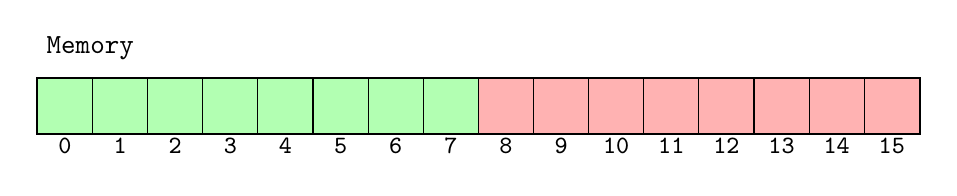
\begin{tikzpicture}[%
    arraynode/.style={
        draw,
        node contents={[\the\numexpr\pgfmatrixcurrentrow-2\relax][\the\numexpr\pgfmatrixcurrentcolumn-2\relax]},
        alias=n\the\numexpr\pgfmatrixcurrentrow-2\relax\the\numexpr\pgfmatrixcurrentcolumn-2\relax
        },
    columnlabel/.style={
        minimum size=0pt,
        draw=none,
        red,
        node contents={\the\numexpr\pgfmatrixcurrentcolumn-2\relax},
        alias=c\the\numexpr\pgfmatrixcurrentcolumn-2\relax
        },      
    rowlabel/.style={
        minimum size=0pt,
        draw=none,
        red,
        node contents={\the\numexpr\pgfmatrixcurrentrow-2\relax},
        alias=r\the\numexpr\pgfmatrixcurrentrow-2\relax
        },      
    emptynode/.style={node contents=~, draw=none},
    font=\ttfamily,
    array/.style={%
        matrix of nodes,
        nodes = arraynode,
        column sep=-\pgflinewidth,
        row sep=-\pgflinewidth, 
        nodes in empty cells,
        row 1/.style={nodes=columnlabel},
        column 1/.style={nodes=rowlabel},
        row 1 column 1/.style={%
            nodes=emptynode}}, 
    rowlabel2/.style={
        inner sep=2pt,
        draw=none,
        font=\small\ttfamily,
        node contents={\the\numexpr-1+\pgfmatrixcurrentcolumn\relax},
        alias=m\the\numexpr-1+\pgfmatrixcurrentcolumn\relax
        },      
    memoryrow/.style={%
        matrix of nodes,
        row 1/.style={nodes = {draw, minimum size=7mm}},
        column sep=-\pgflinewidth,
        row sep=-\pgflinewidth, 
        nodes in empty cells,
        row 2/.style={nodes=rowlabel2}}, 
    memory/.style={%
        matrix of nodes,
        nodes={draw, minimum size=6mm, anchor=center},
        row 1/.style={nodes = {columnlabel, black}},
        column 1/.style={nodes = {rowlabel, black}},
        row 1 column 1/.style={nodes = emptynode},
        column sep=-\pgflinewidth,
        row sep=-\pgflinewidth, 
        nodes in empty cells,
    } 
]

\begin{scope}[yshift=-4cm]

\matrix[memoryrow] (memrow) {
&&&&&&&&&&&&&&&\\
&&&&&&&&&&&&&&&\\};

\node[above right=1mm and 0 of memrow-1-1.north west] {Memory};
\draw[thick] (memrow-1-1.north west) rectangle (memrow-1-16.south east);

\begin{scope}[on background layer]
\fill[red!30] (memrow-1-9.north west) rectangle (memrow-1-16.south east);
\fill[green!30] (memrow-1-1.north west) rectangle (memrow-1-8.south east);
\end{scope}
\end{scope}

\end{tikzpicture}
\end{center}

Now that we have decided on a safety policy with which to execute $\asprg$, we need to figure out how to actually enforce it in our program. Intuitively, our policy defines a ``bad thing'' that is any memory access outside of the sandbox region defined by upper and lower bounds $s_l, s_h$. So we might reasonably enforce the policy by first checking that the index $i$ of any memory access operation in $\asprg$ satisfies $s_l \le i \le s_h$ before executing the operation. Luckily our language contains $\passert{\ivr}$ commands, which come in handy when implementing such checks: if the check fails, the trace aborts rather than violating the policy.

So taking stock of our language, we propose to do the following \emph{instrumentation} of $\asprg$.
\begin{itemize}
  \item Replace each command of the form $\pderef{\astrm}:=\bstrm$ with a new composed command:
  \[
  \passert{s_l \le \astrm \le s_h}; \pderef{\astrm}:=\bstrm
  \]
  This will ensure that $\asprg$ doesn't update any locations outside the sandbox.

  \item Replace any command $\bsprg$ containing the term $\pderef{\astrm}$ with the command:
  \[
  \passert{s_l \le \astrm \le s_h}; \bsprg
  \]
  This will ensure that $\asprg$ doesn't read any locations outside the sandbox.
\end{itemize}
This seems pretty convincing. Our language is fairly simple, so we're pretty sure that all our bases our covered in terms of sandboxing $\asprg$. The assertions themselves are a straightforward reflection of our sandboxing policy.

The downside to this type of enforcement is that any violation of the sandboxing policy, regardless of whether it is inadvertent or intentionally malicious, will cause our entire program to abort. This is less than ideal, as the malice or incompetence of $\asprg$'s developers still has a direct impact on the functioning of our code. Perhaps we can do better. In the next lecture, we will see how to isolate the rest of our programs from these effects using software fault isolation.

% \bibliographystyle{abbrv}
% \bibliography{bibliography}
\end{document}
